% !TEX root = ../thesis.tex
\thispagestyle{plain}
\chapter*{Extended Abstract}
\label{ch:extended-abstract}

\begin{refsection}

\begin{center}
	\begin{tabular}{p{3cm}p{10cm}}
		Thema: & \thema \\[1ex]
		Kandidat: & \autor \\[1ex]
		Betreuer: & \prueferA \\
		 & Institut für Optische Systeme\\[1ex]
		 & \prueferB \\
		 & \firma \\[1ex]
		Abgabedatum: & \abgabedatum \\[1ex]
		Schlagworte: & \schlagworte \\[1ex]
	\end{tabular}
\end{center}


\section*{Einleitung}

Robotik spielt im industriellen Bereich eine größer werdende Rolle.
Insbesondere das sogenannte Bin-Picking, also das autonome Greifen unsortierter Teile gewinnt zunehmend an Relevanz.
Zur Erkennung der Objekte werden dabei in vielen Fällen CAD-Modelle benötigt, welche jedoch nicht immer vorliegen.
Die Rekonstruktion aus aufgenommenen 3D-Daten bietet daher eine einfache Möglichkeit, diese zu erhalten.
Es wurden verschiedene Ansätze dafür analysiert, verglichen und bewertet.


\section*{Methodik}

Die Pipeline wurde in großen Teilen auf Basis der Point Cloud Library \cite{rusu2011pcl} implementiert.
Um größtmögliche Flexibilität zu erreichen, wurde das Robot Operating System \cite{quigley2009ros} für die Interaktion mit dem Programm eingesetzt.
Zur Aufnahme der 3D-Punktwolken wurden Kameras von Ensenso \cite{ensensoWebsite} verwendet.

Die Segmentierung der Punktwolke wurde sowohl im 3D durch Euclidean Cluster Extraction und Region Growing getestet, als auch im zweidimensionalen Grauwertbild mithilfe des Watershed-Algorithmus.

Um Punktwolken aneinander auszurichten, wurde zunächst eine globale Registrierung durch 4-Point Congruent Sets \cite{aiger2008fpcs} durchgeführt.
Diese wurde anschließend mit Iterative Closest Point \cite{besl1992method} lokal optimiert.

Zur Triangulierung wurde der Poisson-Algorithmus \cite{kazhdan2006poisson} verwendet. Anschließend wurden alle Faces aus dem Mesh entfernt, welche eine gewählte Distanz von der Punktwolke überschritten.


\section*{Ergebnisse}

Zur Evaluation wurde die Cloud-Mesh-Distanz zwischen den Vertices des generierten Meshs und den Faces des Referenzobjekts bestimmt.
Außerdem wurde die inverse Cloud-Mesh-Distanz errechnet, um die Vollständigkeit zu überprüfen.

\begin{figure}[H]
    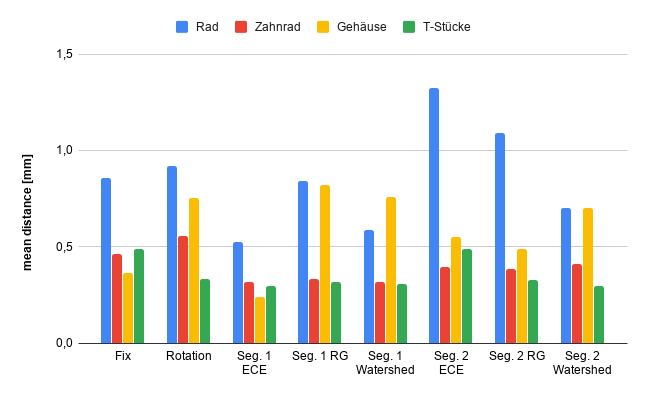
\includegraphics[width=0.49\textwidth]{images/segmentation/meanDistance1.png}
    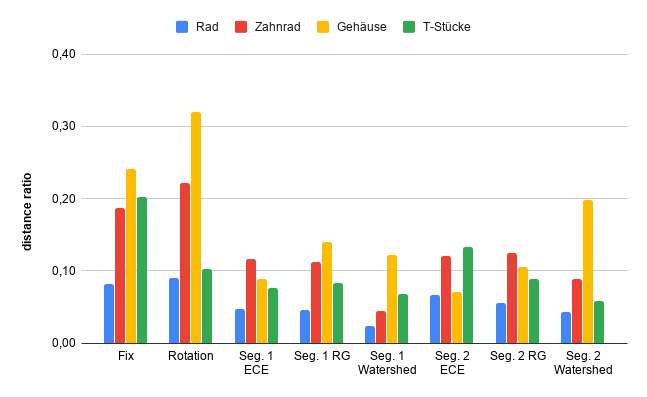
\includegraphics[width=0.49\textwidth]{images/segmentation/ratio.png}
    \caption{Cloud-Mesh-Distanz und Distanzverhältnis verschiedener Testobjekte}
    \label{fig:ex-abstract-distances}
\end{figure}

Es hat sich gezeigt, dass eine Rekonstruktion aus mehreren Aufnahmen eines einzelnen Objekts aus verschiedenen Perspektiven die höchste Qualität erreicht.
In \autoref{fig:ex-abstract-distances} sind die Cloud-Mesh-Distanz von Rekonstruktion zu Referenzobjekt sowie das Distanzverhältnis zu sehen.

Weiterhin ist aufgefallen, dass eine gute Rekonstruktion nur bei korrekter Segmentierung möglich ist.
Bei Untersegmentierung der Punktwolke müssen viele Cluster verworfen werden, während eine korrekte Registrierung bei einer Übersegmentierung oft nicht möglich ist.
Die Wahl der besten Segmentierungsmethode ist abhängig von der Objektform und -größe.


\printbibliography[heading=subbibliography]

\end{refsection}
\newpage
